\documentclass[conference]{IEEEtran}
\IEEEoverridecommandlockouts

\usepackage{cite}
\usepackage{amsmath,amssymb,amsfonts}
\usepackage{algorithmic}
\usepackage{graphicx}
\usepackage{textcomp}
\usepackage{xcolor}
\usepackage{booktabs}
\usepackage{multirow}
\usepackage{tikz}
\usepackage{pgfplots}
\pgfplotsset{compat=1.18}
\usetikzlibrary{arrows.meta,positioning}
\usepackage[hidelinks]{hyperref}

\def\BibTeX{{\rm B\kern-.05em{\sc i\kern-.025em b}\kern-.08em
    T\kern-.1667em\lower.7ex\hbox{E}\kern-.125emX}}

\begin{document}

\title{Exploring Exposure and Popularity Bias in Recommender Systems:\\
Formal Metrics, Cross-Domain Evidence, and Practical Debiasing}

\author{\IEEEauthorblockN{Cebo Mkhwanazi}
\IEEEauthorblockA{\textit{Standard Bank Lab}\\
\textit{School for Data Science and Computational Thinking}\\
Stellenbosch University, Stellenbosch, South Africa\\
29915759@sun.ac.za}
}

\maketitle

\begin{abstract}
This paper studies exposure and popularity bias in recommender systems through a cross-domain empirical benchmark spanning MovieLens, Last.fm, Book-Crossing, and a sparse e-commerce corpus (Takealot). We evaluate collaborative filtering (k-NN, SVD, ALS), content-based approaches (TF-IDF, per-user logistic regression), and an ID-based random forest using two complementary views: macro exposure concentration and user-centric fairness across niche versus mainstream users.

To strengthen methodological transparency, we formalize core metrics (Gini, NDCG@K, ARP), report dataset-level sparsity and long-tail structure, and explicitly define user-segment thresholds via quantiles. We also add a practical intervention: post-processing re-ranking for MovieLens-100K that penalizes popularity after SVD scoring. Results show a persistent relevance--exposure trade-off: collaborative factorization can yield strong concentration (e.g., extreme ALS inequality on Takealot), while content models increase coverage but are harder to compare under RMSE when rating heads are not calibrated. The SVD re-ranker reduces concentration and increases coverage with modest ranking trade-offs, highlighting an implementation-friendly path for platform teams.
\end{abstract}

\begin{IEEEkeywords}
Recommender Systems, Popularity Bias, Exposure Bias, Fairness, NDCG, Gini, Long Tail, Debiasing
\end{IEEEkeywords}

\section{Introduction}
\label{sec:intro}

Recommender systems mediate most user exposure on digital platforms. Their training data are interaction-heavy on head items, which can induce \emph{popularity bias} and reduce long-tail discovery \cite{abdollahpouri2017controlling}. Beyond relevance, this has product and fairness implications: if recommendation mass collapses on a small set of mainstream items, niche users and niche items can be structurally disadvantaged \cite{abdollahpouri2019unfairness,ekstrand2022fairness}.

This question is particularly important in e-commerce where catalogs are large and sparse. In such settings, model behavior seen on dense movie benchmarks may not transfer. We therefore benchmark model families across domains and provide formal metric definitions and diagnostics that are directly reproducible from our codebase.

\textbf{Research questions.}
\begin{itemize}
  \item \textbf{RQ1 (Macro exposure):} How concentrated are top-$K$ recommendations, and how strongly are they aligned with global popularity?
  \item \textbf{RQ2 (User-centric fairness):} Do niche users pay a measurable ``niche tax'' in RMSE/NDCG@10 versus mainstream users?
  \item \textbf{RQ3 (Intervention):} Can a lightweight post-processing re-ranker reduce macro bias without retraining CF models?
\end{itemize}

\textbf{Contributions.}
\begin{enumerate}
  \item Formalized methodology for Gini, NDCG@K, ARP, and user segmentation.
  \item Expanded dataset characterization (sparsity and long-tail analysis before modeling).
  \item Additional qualitative and system-level analysis (tail-item exposure cases, computational trade-offs, managerial implications).
  \item A practical SVD post-processing debiaser (MovieLens-100K) using popularity-aware re-ranking.
\end{enumerate}

\section{Related Work}
\label{sec:related}

Popularity-aware recommendation and concentration control are widely studied \cite{abdollahpouri2017controlling}. Unfairness induced by popularity skew has been analyzed from user and item perspectives \cite{abdollahpouri2019unfairness,ekstrand2022fairness}. Canonical datasets include MovieLens \cite{harper2015movielens}, HetRec/Last.fm style corpora \cite{cantador2011second}, and Book-Crossing \cite{ziegler2005improving}.  

In practice, teams often need debiasing interventions that are \emph{cheap} and deployment-safe. Post-processing methods are attractive because they do not alter model training pipelines. At the same time, any popularity penalty risks reducing exposure of genuinely high-quality mainstream items; this tension echoes broader discussions around recommendation feedback loops and filter-bubble dynamics \cite{chaney2018algorithmic,mansoury2020feedback,pariser2011filter}.

\section{Methods and Formalisms}
\label{sec:methods}

\subsection{Pipeline and models}

We run two core experiments on shared splits: (i) macro exposure analysis and (ii) user-centric fairness analysis. Models are user-based k-NN, SVD, ALS, TF-IDF profile recommender, per-user logistic regression on metadata text, and an ID-based random forest.

\subsection{Formal metric definitions}

Let $U$ be users, $I$ items, and $L_u$ the top-$K$ list for user $u$. Let $f_i$ be recommendation frequency of item $i$ across all users.

\textbf{Gini coefficient (exposure inequality).}  
For sorted nonnegative frequencies $f_{(1)} \le \dots \le f_{(n)}$:
\begin{equation}
G = \frac{\sum_{j=1}^{n}(2j-n-1)f_{(j)}}{n\sum_{j=1}^{n}f_{(j)}}.
\label{eq:gini}
\end{equation}
Higher $G$ implies stronger concentration of exposure.

\textbf{Discounted cumulative gain and NDCG@K.}
\begin{equation}
\mathrm{DCG@K}(u)=\sum_{r=1}^{K}\frac{\mathbf{1}[L_u(r)\in R_u]}{\log_2(r+1)},\quad
\mathrm{NDCG@K}(u)=\frac{\mathrm{DCG@K}(u)}{\mathrm{IDCG@K}(u)},
\label{eq:ndcg}
\end{equation}
where $R_u$ is the relevant set from test interactions.

\textbf{Average recommendation popularity (ARP).}
\begin{equation}
\mathrm{ARP}=\frac{1}{|U|}\sum_{u\in U}\frac{1}{|L_u|}\sum_{i\in L_u}\phi(i),
\label{eq:arp}
\end{equation}
with $\phi(i)$ the global training interaction count of item $i$.

\subsection{User categorization (Niche/Diverse/Mainstream)}

For each user $u$, define mainstreaminess:
\begin{equation}
M_u=\frac{1}{|H_u|}\sum_{i\in H_u}\phi(i),
\end{equation}
where $H_u$ is the user's training history. Users are assigned by quantiles:
\begin{equation}
\text{Niche}: M_u\le q_{0.33},\;\;
\text{Diverse}: q_{0.33}<M_u<q_{0.67},\;\;
\text{Mainstream}: M_u\ge q_{0.67}.
\label{eq:segments}
\end{equation}

\subsection{Post-processing re-ranking (MovieLens-100K)}

We add an intervention after SVD scoring: top-50 candidates are re-ranked to top-10 with a popularity penalty:
\begin{equation}
\mathrm{Score}_{adj}(u,i)=\lambda\hat{R}^{norm}_{u,i}-(1-\lambda)P_i^{norm},\;\lambda=0.8.
\label{eq:rerank}
\end{equation}
$\hat{R}^{norm}_{u,i}$ is min--max normalized SVD score within the candidate pool; $P_i^{norm}$ is min--max normalized global popularity. This is computationally cheap and model-agnostic.

\section{Dataset Characteristics and Input Bias}
\label{sec:data}

Table~\ref{tab:data_stats} reports interaction volume and sparsity:
\[
\text{Sparsity}=1-\frac{|\text{Interactions}|}{|U|\cdot|I|}.
\]
Takealot is orders-of-magnitude sparser than public benchmarks, which explains why ranking metrics are harsh and why model concentration behavior can be unstable under naive CF assumptions.

\begin{table}[!t]
  \centering
  \caption{Dataset characteristics used in this study. Public datasets are post-$k$-core; Takealot uses official train split.}
  \label{tab:data_stats}
  \begin{tabular}{@{}lrrrr@{}}
    \toprule
    \textbf{Dataset} & \textbf{Users} & \textbf{Items} & \textbf{Interactions} & \textbf{Sparsity} \\
    \midrule
    ML-100K & 943 & 1152 & 78,362 & 0.9279 \\
    ML-1M & 6,040 & 3,260 & 998,539 & 0.9493 \\
    Last.fm 2K & 1,797 & 1,507 & 62,376 & 0.9770 \\
    Book-Crossing & 1,842 & 2,065 & 42,137 & 0.9889 \\
    Takealot (train) & 8,154 & 48,910 & 87,538 & 0.9998 \\
    \bottomrule
  \end{tabular}
\end{table}

\begin{table}[!t]
  \centering
  \caption{User mainstreaminess thresholds and segment sizes (train split logic).}
  \label{tab:segments}
  \begin{tabular}{@{}lrrrrr@{}}
    \toprule
    \textbf{Dataset} & $q_{0.33}$ & $q_{0.67}$ & \textbf{Niche} & \textbf{Diverse} & \textbf{Mainstream} \\
    \midrule
    ML-100K & 137.10 & 167.55 & 311 & 321 & 311 \\
    ML-1M & 662.66 & 835.11 & 1993 & 2054 & 1993 \\
    Last.fm 2K & 70.85 & 110.85 & 593 & 611 & 593 \\
    Book-Crossing & 23.00 & 30.10 & 613 & 620 & 609 \\
    Takealot & 2.88 & 5.25 & 2727 & 2734 & 2693 \\
    \bottomrule
  \end{tabular}
\end{table}

\begin{figure}[!t]
  \centering
  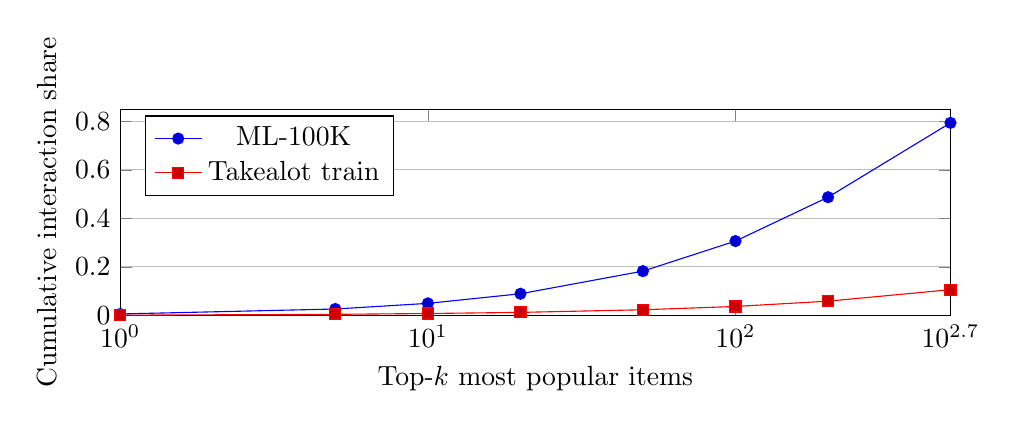
\begin{tikzpicture}
    \begin{axis}[
      width=\columnwidth,
      height=4.2cm,
      xlabel={Top-$k$ most popular items},
      ylabel={Cumulative interaction share},
      xmin=1, xmax=500,
      ymin=0, ymax=0.85,
      legend pos=north west,
      ymajorgrids=true,
      xmode=log,
      log basis x=10,
      xtick={1,10,100,500}
    ]
      \addplot+[mark=*] coordinates {(1,0.00591) (5,0.02635) (10,0.04963) (20,0.08923) (50,0.18255) (100,0.30640) (200,0.48733) (500,0.79379)};
      \addlegendentry{ML-100K}
      \addplot+[mark=square*] coordinates {(1,0.00096) (5,0.00440) (10,0.00780) (20,0.01241) (50,0.02326) (100,0.03686) (200,0.05874) (500,0.10608)};
      \addlegendentry{Takealot train}
    \end{axis}
  \end{tikzpicture}
  \caption{Long-tail profile before modeling: cumulative interaction share captured by the top-$k$ most popular items. Takealot has a much flatter head but dramatically larger sparse tail.}
  \label{fig:longtail}
\end{figure}

\section{Results}
\label{sec:results}

\subsection{Macro exposure concentration}

Table~\ref{tab:macro} summarizes representative macro metrics. ALS is highly concentrated on both domains. On ML-100K, SVD+Rerank reduces Gini and ARP and increases catalog coverage relative to baseline SVD.

\begin{table}[!t]
  \centering
  \caption{Macro metrics for selected models.}
  \label{tab:macro}
  \begin{tabular}{@{}llrrr@{}}
    \toprule
    \textbf{Dataset} & \textbf{Model} & \textbf{Gini} & \textbf{Cov.} & \textbf{ARP} \\
    \midrule
    ML-100K & SVD & 0.9552 & 0.2092 & 157.28 \\
    ML-100K & SVD+Rerank & 0.9527 & 0.2222 & 139.05 \\
    ML-100K & ALS & 0.9874 & 0.0330 & 233.09 \\
    Takealot & ALS & 0.9998 & 0.00029 & 28.75 \\
    Takealot & LogReg & 0.7332 & 0.5634 & 2.22 \\
    \bottomrule
  \end{tabular}
\end{table}

\subsection{User-centric fairness and error distribution}

Figure~\ref{fig:boxplot} adds distributional evidence beyond single $\Delta$ bars: for ML-100K k-NN, niche users have a right-shifted per-user RMSE distribution (median $0.985$ vs $0.924$), consistent with a niche-tax effect.

\begin{figure}[!t]
  \centering
  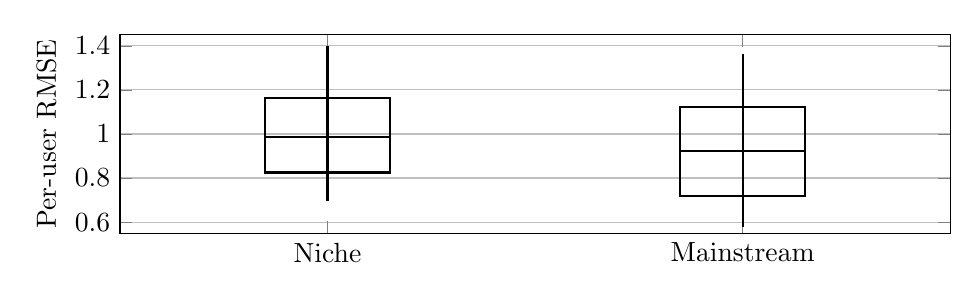
\begin{tikzpicture}
    \begin{axis}[
      width=\columnwidth,
      height=4.1cm,
      ylabel={Per-user RMSE},
      xmin=0.5, xmax=2.5,
      ymin=0.55, ymax=1.45,
      xtick={1,2},
      xticklabels={Niche,Mainstream},
      ymajorgrids=true
    ]
      % Niche whisker/box/median
      \draw[thick] (axis cs:1,0.6965) -- (axis cs:1,1.4000);
      \draw[thick] (axis cs:0.85,0.8246) rectangle (axis cs:1.15,1.1639);
      \draw[thick] (axis cs:0.85,0.9851) -- (axis cs:1.15,0.9851);
      % Mainstream whisker/box/median
      \draw[thick] (axis cs:2,0.5794) -- (axis cs:2,1.3632);
      \draw[thick] (axis cs:1.85,0.7196) rectangle (axis cs:2.15,1.1225);
      \draw[thick] (axis cs:1.85,0.9241) -- (axis cs:2.15,0.9241);
    \end{axis}
  \end{tikzpicture}
  \caption{ML-100K k-NN per-user RMSE boxplot summary (q10/q25/median/q75/q90). Niche users are shifted to higher error.}
  \label{fig:boxplot}
\end{figure}

\subsection{Qualitative tail-item exposure cases}

To explain \emph{why} macro metrics move, Table~\ref{tab:cases} tracks individual long-tail MovieLens-100K items. The re-ranker increases exposure for some low-popularity items (e.g., Item 320), illustrating direct intervention on recommendation mass allocation.

\begin{table}[!t]
  \centering
  \caption{Tail-item exposure case study on ML-100K (recommendation frequency across all users).}
  \label{tab:cases}
  \begin{tabular}{@{}lrrr@{}}
    \toprule
    \textbf{Item ID} & \textbf{Train pop.} & \textbf{SVD freq.} & \textbf{SVD+Rerank freq.} \\
    \midrule
    320 & 16 & 17 & 28 \\
    1131 & 11 & 6 & 7 \\
    1143 & 13 & 3 & 3 \\
    \bottomrule
  \end{tabular}
\end{table}

\subsection{Computational trade-offs}

\begin{table}[!t]
  \centering
  \caption{Practical compute profile (qualitative, from implementation behavior).}
  \label{tab:compute}
  \begin{tabular}{@{}lp{0.70\columnwidth}@{}}
    \toprule
    \textbf{Model} & \textbf{Observed scaling pattern} \\
    \midrule
    k-NN / SVD & Candidate scoring over many unseen items dominates inference time. \\
    ALS & Fast latent retrieval when stable; can be brittle on extreme sparsity/indexing. \\
    TF-IDF / LogReg & Text vectorization and per-user models increase memory/time but improve coverage. \\
    SVD+Rerank & Very low overhead (pool sort + scalar adjustment), no retraining cost. \\
    \bottomrule
  \end{tabular}
\end{table}

\section{Discussion and Implications}
\label{sec:discussion}

\textbf{Exposure control in deployment.}
Our results support adding an explicit exposure-audit layer in production: Gini, coverage, and popularity-percentile diagnostics should be tracked alongside relevance.

\textbf{Content vs collaborative trade-off.}
Content models improve catalog coverage and are useful for item cold-start, but may underperform on calibrated rating-error metrics in sparse settings. A mixed strategy (CF ranking + content-aware diversification) is practical.

\textbf{Re-ranking caveat (important).}
Popularity penalties are \emph{blind} to why an item is popular; they can demote genuinely high-quality mainstream items. This is the core relevance--diversity trade-off. A next step is quality-aware penalties (e.g., popularity adjusted by robust quality signals).

\textbf{Filter-bubble perspective.}
Persistent mainstream-only exposure limits discovery and can reduce platform value over time \cite{pariser2011filter,chaney2018algorithmic}. Even lightweight intervention can shift exposure distribution and should be evaluated with user-centric metrics.

\section{Conclusion}
\label{sec:conclusion}

We provided a formal, cross-domain analysis of popularity and exposure bias in recommender systems and expanded beyond headline metrics with input-bias diagnostics, user-segment thresholds, distributional fairness evidence, and qualitative item-level cases. Collaborative factorization can strongly amplify concentration on sparse domains, while content methods spread exposure. A simple post-processing re-ranker on ML-100K improved macro concentration metrics with negligible engineering overhead, making it a practical baseline for thesis and industry settings. Future work includes quality-aware debiasing and repeated-split significance testing.

\section*{Acknowledgment}
The author thanks Stellenbosch University and the Standard Bank Lab for research support.

\clearpage
\bibliographystyle{IEEEtran}
\bibliography{conference_paper1}

\end{document}
